\question{Câu 2}

 Cho mạch khuếch đại tín hiệu như hình vẽ. Các tụ $C_{1}$, $C_{2}$ có giá trị rất lớn. BJT có hệ số $\beta = 80$ và có mã là 2N2907.
 
 \begin{figure}[H]
 	\centering
	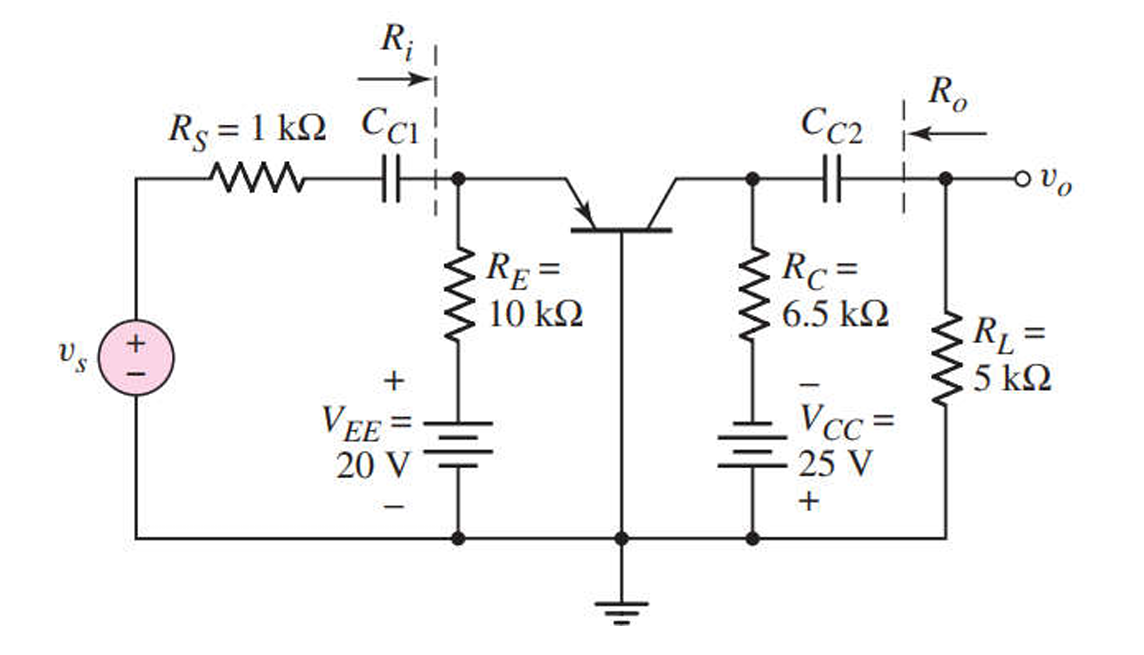
\includegraphics[width=.8\linewidth]{./my-chapters/my-images/Question2/debai.png}
 \end{figure}
 
\answer{a}{Vẽ VTC của mạch (kiểm chứng sử dụng mô phỏng) và tìm điểm hoạt động $Q$ của BJT.}

Vẽ VTC của mạch:

\begin{itemize}[label=-]
	\item $v_{EB}<V_{EB(ON)}$: BJT hoạt động ở trạng thái \textbf{cut-off}  
	\[
	\Rightarrow i_{C}=0 \Rightarrow V_{C}=-V_{CC}=-25\,\textsf{V}
	\]
	
	\item $v_{EB}=V_{EB(ON)}=0.7\,\textsf{V}$: BJT hoạt động ở trạng thái \textbf{active}  
	\[
	V_{i}=V_{E}=V_{B}+V_{BE(ON)}=0+0.7=0.7\,\textsf{V}
	\]
	\[
	V_{o}=V_{i}-V_{CEsat}=0.7-0.2=0.5\,\textsf{V}
	\]
	\[
	I_{C}=\beta I_{B}
	\]
	
	\item $v_{EB}\geq\left.V_{EB}\right|_{v_{EC}={v_{EC}}_{sat}}$: BJT hoạt động ở trạng thái \textbf{saturation}  
	\[
	v_{EC}={v_{EC}}_{sat}=0.2\,\textsf{V}
	\]
	\[
	\Rightarrow V_{EC}=(V_{EE}+V_{CC})-I_{E}(R_{E}+R_{C})
	\]
	\[
	\Rightarrow 0.2=(20+25)-I_{E(sat)}(10\,\textsf{k}+6.5\,\textsf{k})
	\]
	\[
	\Rightarrow I_{E(sat)}=2.715\,\textsf{mA}
	\]
\end{itemize}

Tìm \textbf{điểm hoạt động Q}:

Giả sử BJT hoạt động ở chế độ khuếch đại:
\[
V_{E}=V_{B}+V_{EB}=0+0.7=0.7\,\textsf{V}
\]

Áp dụng KVL cho vòng 1:
\[
- V_{EE}+R_{E}I_{E}+V_{EB}=0
\]
\[
\Rightarrow I_{E}=\frac{V_{EE}-V_{EB}}{R_{E}}=\frac{20-0.7}{10\,\textsf{k}}=1.93\,\textsf{mA}
\]
\[
\Rightarrow I_{C}=\frac{\beta}{\beta+1}\times I_{E}=1.906\,\textsf{mA}
\]

Áp dụng KVL cho vòng 2:
\[
- V_{EE}+I_{E}(R_{E}+R_{C})+V_{EC}-V_{CC}=0
\]
\[
\Rightarrow V_{EC}=13.155\,\textsf{V}
\]

Vậy điểm làm việc $Q$ là: \finalresult{\left(I_{CQ},V_{ECQ}\right)=\left(1.93\,\textsf{mA},\,13.155\,\textsf{V}\right)}.

\answer{b}{Đặt $v_{1} = V_{m} \sin \left( \omega t\right)$ vào mạch. Tìm $A_{vo}$, $G_v$, $R_i$, $R_o$ của mạch.}

\[
g_{m}=\frac{I_{C}}{V_{T}}=0.07624\,\textsf{mS}
\]
$\Rightarrow$ \finalresult{g_{m}=0.07624\,\textsf{mS}}.

\[
R_{i}=\frac{1}{g_{m}}\,//\,R_{E}=\frac{\frac{1}{0.07624}\times10\,\textsf{k}}{\frac{1}{0.07624}+10\,\textsf{k}}=13.1\,\Omega
\]
$\Rightarrow$ \finalresult{R_{i}=13.1\,\Omega}.

\[
R_{o}=R_{C}=6.5\,\textsf{k}\Omega
\]
$\Rightarrow$ \finalresult{R_{o}=6.5\,\textsf{k}\Omega}.

\[
A_{vo}=g_{m}R_{C}=495.56\,\textsf{V/V}
\]
$\Rightarrow$ \finalresult{A_{vo}=495.56\,\textsf{V/V}}.

\[
A_{v}=A_{vo}\times\frac{R_{L}}{R_{o}+R_{L}}=495.56\times\frac{5\,\textsf{k}}{5\,\textsf{k}+6.5\,\textsf{k}}=215.46\,\textsf{V/V}
\]
$\Rightarrow$ \finalresult{A_{v}=215.46\,\textsf{V/V}}.

\[
G_{v}=A_{vo}\times\frac{R_{L}}{R_{o}+R_{L}}\times\frac{R_{i}}{R_{sig}+R_{i}}=495.56\times\frac{5\,\textsf{k}}{5\,\textsf{k}+6.5\,\textsf{k}}\times\frac{13.1}{1\,\textsf{k}+13.1}=2.79\,\textsf{V/V}
\]
$\Rightarrow$ \finalresult{G_{v}=2.79\,\textsf{V/V}}.

\answer{c}{Lựa chọn các tụ $C_{1}$, $C_{2}$ để mạch có $f_{L}=100\,\textsf{Hz}$.}

\begin{itemize}[label=-]
	\item Xét ảnh hưởng tụ $C_{1}$: 
	\[
	R_{C_{1}} = R_{sig} \,||\, R_{in}
	\Longrightarrow 
	\omega_{p_{1}} = \frac{1}{C_{1}\left(R_{sig} \,||\, R_{in}\right)}
	\]
	
	\item Xét ảnh hưởng tụ $C_{2}$: 
	\[
	R_{C_{2}} = R_{C} + R_{L}
	\Longrightarrow 
	\omega_{p_{2}} = \frac{1}{C_{2}\left(R_{C} + R_{L}\right)}
	\]
\end{itemize}

Theo phương pháp \textbf{cực tần số trội (dominant pole)}, chọn $C_{1}$ làm cực trội có giá trị $100\,\textsf{Hz}$, 
$C_{2}$ tạo ra cực ở tần số $40\,\textsf{Hz}$.  
Như vậy, tần số cắt của mạch là:
\[
f_{L} = \sqrt{f_{C_{1}}^{2} + f_{C_{2}}^{2}}
\]

\textbf{Lựa chọn các tụ $C_{1}$ và $C_{2}$:}
\[
C_{1} = \frac{1}{2\pi \times 100 \times (1\,\textsf{k}\,||\,13.1\,\textsf{k})}
= 123.08\,\mu\textsf{F}
\]
\[
C_{2} = \frac{1}{2\pi \times 40 \times (6.5\,\textsf{k} + 5\,\textsf{k})}
= 0.36\,\mu\textsf{F}
\]

$\Rightarrow$ \finalresult{C_{1} = 123.08\,\mu\textsf{F}} và \finalresult{C_{2} = 0.36\,\mu\textsf{F}}.
